\documentclass [10pt, a4paper]{article}

\usepackage{graphicx}
% \usepackage[margin=1in]{geometry}
\usepackage{fancyhdr}
\usepackage {float}
\newfloat {diagram}{thp}{lop}
\floatname{diagram}{Diagram}

\usepackage {verbatim}

\oddsidemargin 0cm
\topmargin -2cm
\textwidth 16.5cm
\textheight 23.5cm

\pagestyle{fancyplain}
\lhead{\fancyplain{}{\textbf{P1 Design doc}}}
\rhead{\fancyplain{}{El-Hassan Wanas\\ ewanas}}
\chead{\fancyplain{}{15-440}}

\title {P1 Design document}
\author {El-Hassan Wanas\\ewanas@qatar.cmu.edu}

\begin {document}
\maketitle

\section {Starter code overview}
This section describes the starter code structure and the way I plan to approach
this project.

\begin {diagram}
\begin {center}
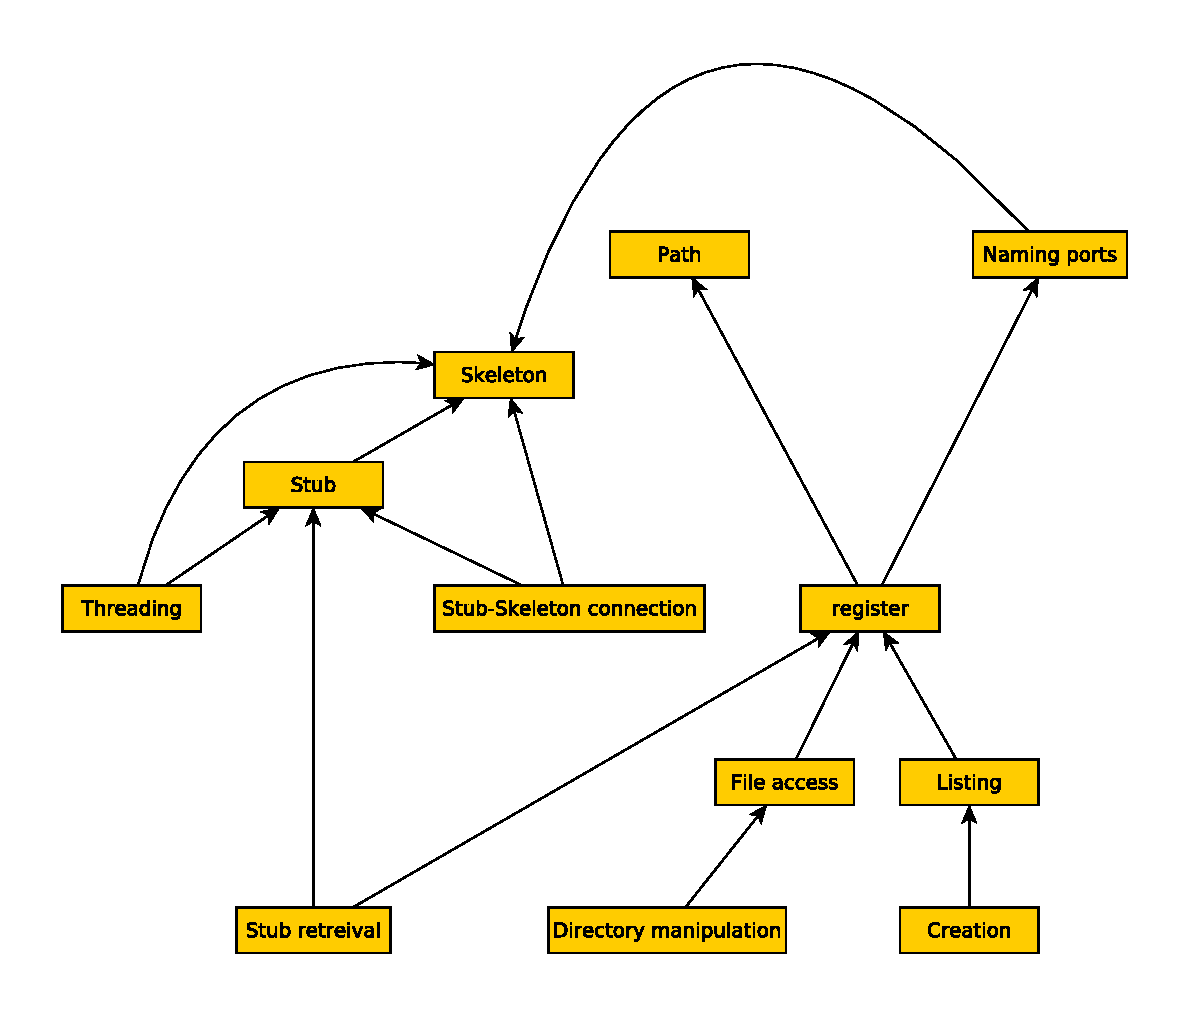
\includegraphics[scale=0.6]{sequence.eps}
\end {center}
\caption {Module dependancy}
\end {diagram}

\subsection {RMI}
\subsubsection {Skeleton}
A \texttt{Skeleton} serves implementations of interfaces to \texttt{Stub}
factories. The main point behind the \texttt{Skeleton} is to allow different
implementations of
the same interface to reside on multiple machines and not having to change the
client code to be able to use those implementations.

In File Stack, we will be running two skeletons. One on the naming server and
one on the storage server. The skeleton on the naming server will serve
implementations of the File Stack interface to clients. The skeleton on the
storage server will serve implementations of the \texttt{Storage} interface to
the naming server.

\subsubsection {Stub}
A \texttt{Stub} is really an interface that isn't yet implemented, but which you
request an implementation for. The convenient Stub factory should hide all the
details of obtaining the implementation.

\subsection {Naming}
The \texttt{naming server}'s mission is twofold. For one, it should accept
\texttt{storage server}
requests and requests from clients. It keeps track of which files belong to
which servers and it forwards \texttt{storage server} stub
implementations to clients, upon invoking an operation on a file.

When a storage server connects to the naming server, the naming server should
receive an implementation of the Storage interface.

\begin {diagram}
\begin {center}
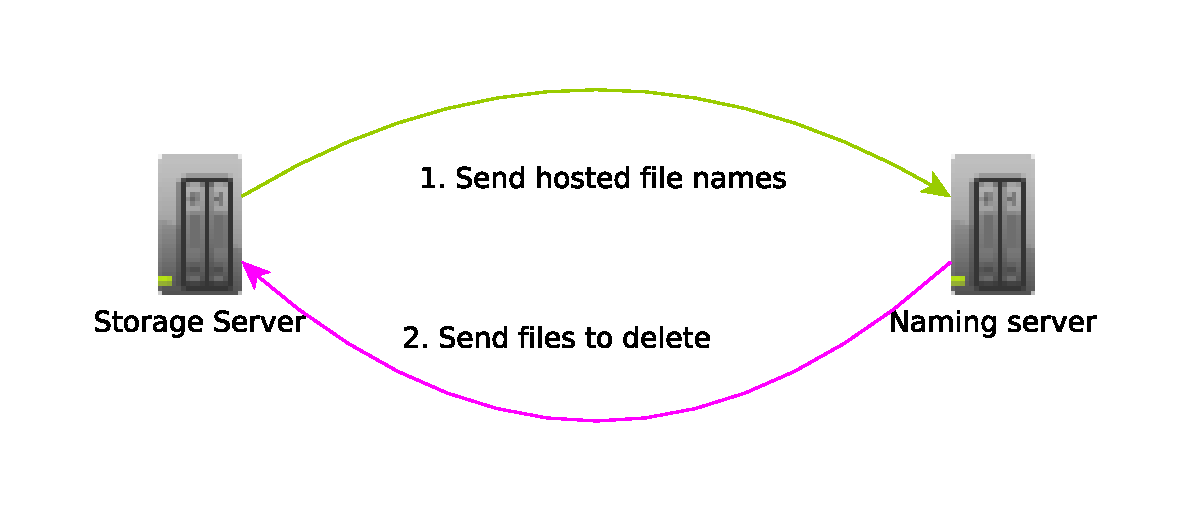
\includegraphics[scale=0.6]{register.eps}
\end {center}
\caption {Registration}
\end {diagram}
\begin {diagram}
\begin {center}
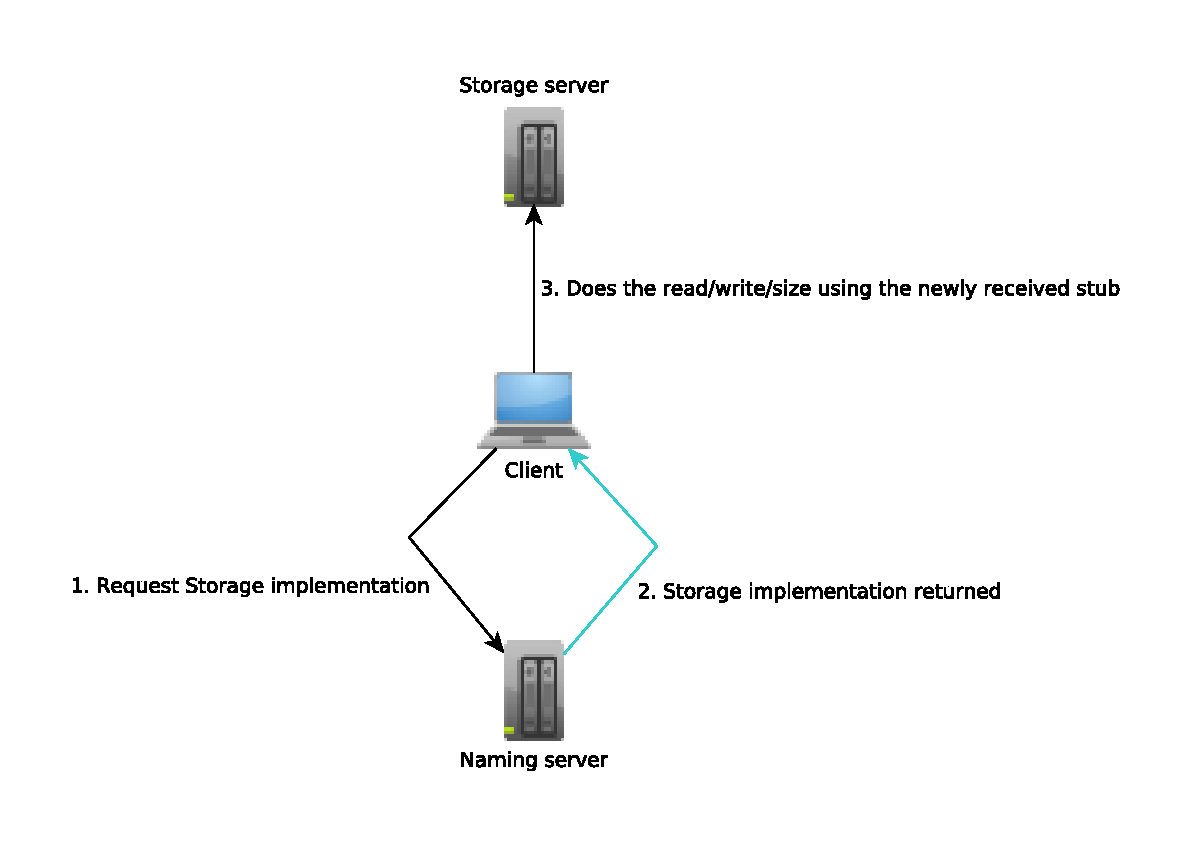
\includegraphics[scale=0.6]{naming.eps}
\end {center}
\caption {Client read/write/size implementation}
\end {diagram}
\begin {diagram}
\begin {center}
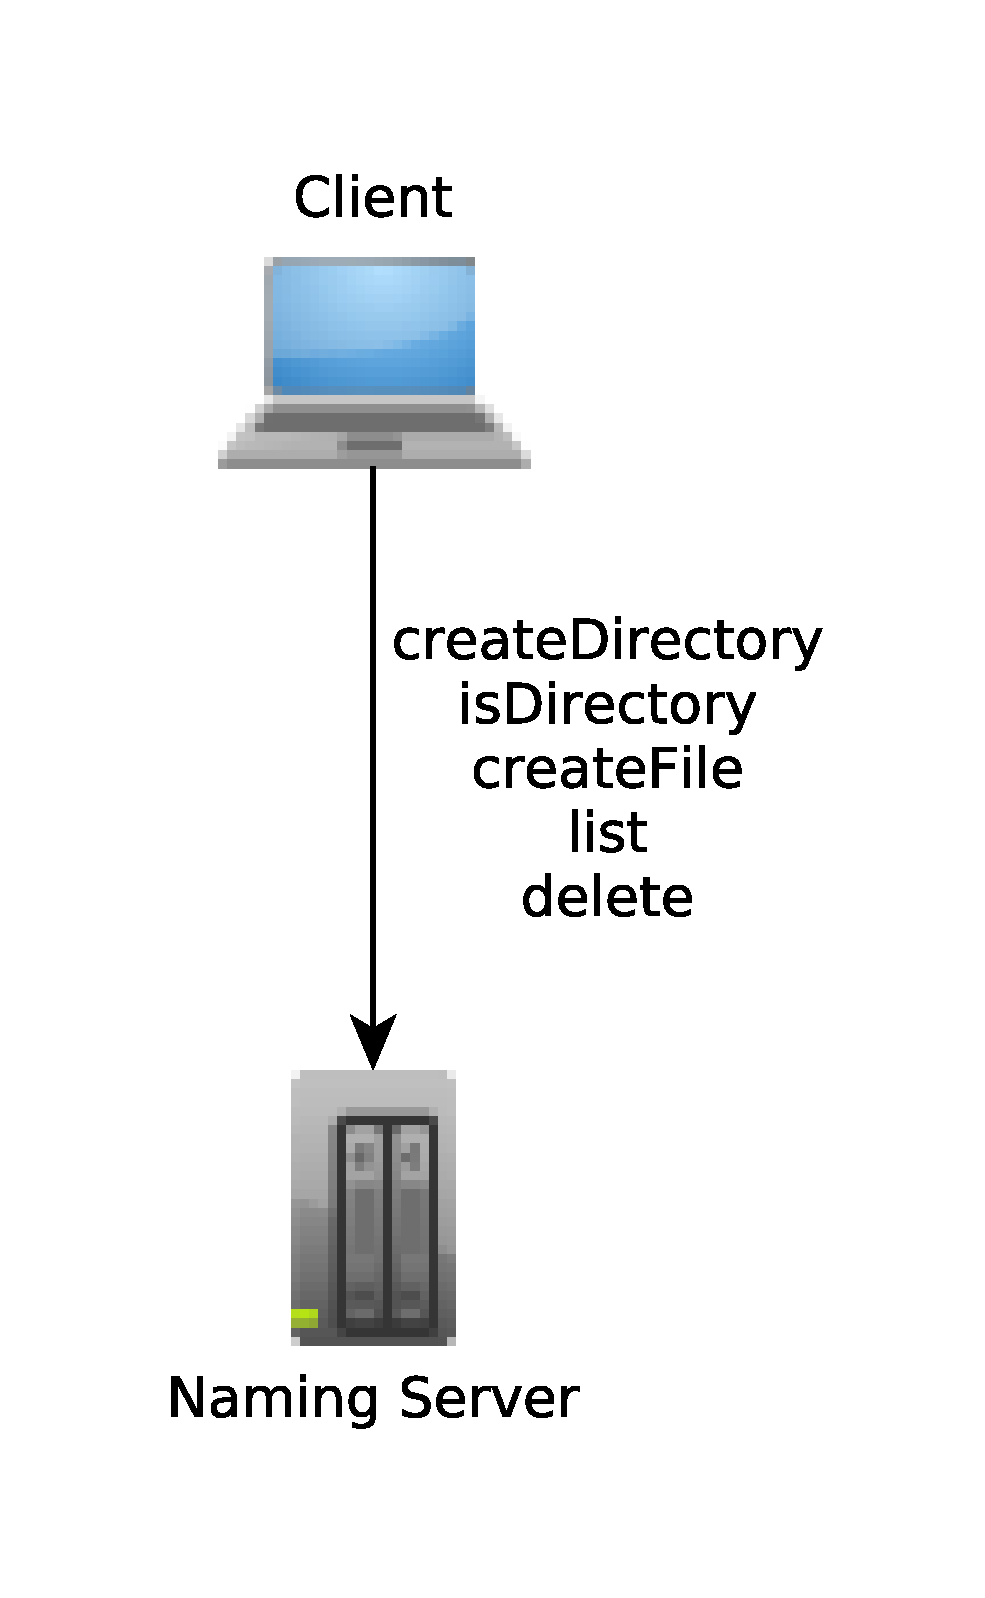
\includegraphics[scale=0.2]{naming-client.eps}
\end {center}
\caption {Client meta file operations}
\end {diagram}

\newpage

\subsection {Storage}
Storage servers connect to naming servers, to bring forth their share of the
file system to view. They will get connections from clients beyond that. When
the client wants to read/write/size it should first ask the server for the
actual implementation of \texttt{Storage} that will support the operation and
hide the actual storage server. The communication after receiving that
implementation happens between the client and the storage server only.

\section {Logic of unimplemented functionalities}

I would probably want to use ExecutorService to manage my threads, for this
project. It has a very convenient way of managing a thread pool.

\subsection {Skeleton}

\subsubsection {\texttt{public Skeleton(Class<T> c, T server)}}
Listen on a random port for requests for implementations of the interface $c$.

\subsubsection {\texttt{public Skeleton(Class<T> c, T server, InetSocketAddress
address)}}
Listen on a specific port for requests for implementations of the interface $c$.

\subsubsection {\texttt{public synchronized void start() throws RMIException}}
Starts the server on a seperate thread. For every new connection, a new thread
is created.

\subsubsection {\texttt{public synchronized void stop()}}
Stop the main server thread.

\subsection {Stub}

\subsubsection {\texttt{public static <T> T create(Class<T> c, Skeleton<T>
skeleton) throws UnknownHostException}}
Connect to the skeleton and requests an implementation of the interface
designated by the type $T$.

\subsubsection{\texttt{public static <T> T create(Class<T> c, Skeleton<T>
skeleton, String hostname)}}
Connect to the skeleton of type Skeleton T running at another host and request
for an implementation of the interface designated by the type $T$.

\subsubsection{\texttt{public static <T> T create(Class<T> c, InetSocketAddress
address)}}
Connect to the server at the given hostname and port and requests an
implementation of the interface $T$.

\subsection {NamingServer}

\subsubsection{\texttt{public NamingServer()}}
Does nothing special, as far as I can tell at this point.

\subsubsection{\texttt{public synchronized void start() throws RMIException}}
Create a ServerSocket in a new thread and start listening for requests.

\subsubsection{\texttt{public void stop()}}
Terminate all threads created by the NamingServer.

\subsubsection{\texttt{@Override public boolean isDirectory(Path path) throws
FileNotFoundException}}
Look up the permissions for the path in the Map<Path,Permissions> that will be
created within the NamingServer.

\subsubsection{\texttt{@Override public String[] list(Path directory) throws
FileNotFoundException}}
Return all the keys in the Map<Path,Permissions>.

\subsubsection{\texttt{@Override public boolean createFile(Path file) throws
RMIException, FileNotFoundException}}
Use one of the storage server implementations to create the file and add it to
the global Map<Path,Permissions>.

\subsubsection{\texttt{@Override public boolean createDirectory(Path directory)
throws FileNotFoundException}}
Use one of the storage server implementations to create the file and add it to
the global Map<Path,Permissions>.

\subsubsection{\texttt{@Override public boolean delete(Path path) throws
FileNotFoundException}}
Use one of the storage server implementations to delete the file and remove it
from the global Map<Path,Permissions>.

\subsubsection{\texttt{@Override public Storage getStorage(Path file) throws
FileNotFoundException}}
Return the value in the Map<Path,Storage> for the key with value file.

\subsubsection{\texttt{@Override public Path[] register(Storage client\_stub,
Command command\_stub, Path[] files)}}

\subsection {StorageServer}

\subsubsection{\texttt{public StorageServer(File root)}}
Initialize the StorageServer in such a way that the value of root becomes the
prefix to every Path of a file on that server.

\subsubsection{\texttt{public synchronized void start(String hostname,
Registration naming\_server)\\ throws RMIException, UnknownHostException,
FileNotFoundException}}
Try to connect to the naming server running at \texttt{hostname} and register
using the value for \texttt{naming\_server}.

\subsubsection{\texttt{public void stop()}}
Terminates all the threads running on the StorageServer.

\subsubsection{\texttt{@Override public synchronized long size(Path file) throws
FileNotFoundException}}
Return the size of the file at root + file.toString ().

\subsubsection{\texttt{@Override public synchronized byte[] read(Path file, long
offset, int length) throws FileNotFoundException, IOException}}
Return the first \texttt{length} bytes after the \texttt{offset} of the file
located at root + file.toString ().

\subsubsection{\texttt{@Override public synchronized void write(Path file, long
offset, byte[] data) throws FileNotFoundException, IOException}}
Overwrites the file at root + file.toString () from offset with the contents of
data.

\subsubsection{\texttt{@Override public synchronized boolean create(Path file)}}
Create a new file at root + file.toString ().

\subsubsection{\texttt{@Override public synchronized boolean delete(Path path)}}
This should lock access to the file at root + path.toString () and delete it.

\subsection {Path}

\subsubsection{\texttt{public Path()}}
\begin {verbatim}
{
}
\end {verbatim}

\subsubsection{\texttt{public Path(Path path, String component)}}
\begin {verbatim}
    {
        if (component == null || !isValid (component)) {
            throw new IllegalArgumentException (
                    "Invalid path component"
                    );
        }

        pathPrefix      = path;
        pathComponent   = component;
    }
\end {verbatim}

\subsubsection{\texttt{public Path(String path)}}
\begin {verbatim}
    {
        String [] components;

        if (path != null && path.indexOf ("/") == 0) {
            path = path.substring (1);

            pathPrefix = new Path ();

            components = path.split ("/");

            if (components.length >= 1) {
                pathComponent = components [components.length - 1];

                components = Arrays.copyOfRange (components, 0,
components.length - 1);

                for (String component : components) {
                    if (!component.equals ("")) {
                        pathPrefix = new Path (pathPrefix, component);
                    }
                }
            } else if (path.equals ("/")) {
                return;
            }

            return;
        }

        throw new IllegalArgumentException (
                "Invalid path string"
                );
    }
\end {verbatim}

\subsubsection{\texttt{@Override public Iterator<String> iterator()}}
\begin {verbatim}
    {
        return new ComponentIterator (this);
    }

    /** The component String iterator.

        <p>
        This iterator will not support <code>remove()</code>. It will throw an
        <code>UnsupportedOperationException</code>, in such cases.
    */
    private class ComponentIterator implements Iterator <String>
    {
        Iterator <String> listIterator;

        /** Creates a new <code>ComponentIterator</code> that goes through
            a list of path components.

            @param path is a <code>Path</code> that this iterator will go
                        through the components of.
        */
        public ComponentIterator (Path path)
        {
            List <String> components = new ArrayList <String> ();

            for (Path p = path; p.pathPrefix != null; p = p.pathPrefix) {
                components.add (0, p.pathComponent);
            }

            listIterator = components.iterator ();
        }

        /** Checks if there are more components in the path.

            @return true if there are more components.
        */
        public boolean hasNext ()
        {
            return listIterator.hasNext ();
        }

        /** Returns the next component in the path.

            @throws NoSuchElementException if there are no more components
                    in the path.
            @return The next component in the path.
        */
        public String next ()
        {
            return listIterator.next ();
        }

        /** Method isn't implemented.

            @throw UnsupportedOperationException Because this method isn't
                                                 implemented.
        */ 
        public void remove ()
        {
            throw new UnsupportedOperationException (
                    "Can't remove component using path component iterator"
                    );
        }
    }
\end {verbatim}

\subsubsection{\texttt{public static Path[] list(File directory) throws
FileNotFoundException}}
\begin {verbatim}
    {
        List <Path> contents    = new ArrayList <Path> ();
        int         length      = directory.toString ().length ();

        if (!directory.exists ()) {
            throw new FileNotFoundException (
                    "File " + directory.getName () + " doesn't exist"
                    );
        } else if (!directory.isDirectory ()) {
            throw new IllegalArgumentException (
                    "Not a directory"
                    );
        } else {
            Queue <File> files = new LinkedList <File> ();
            files.add (directory);

            while (!files.isEmpty ()) {
                File currentFile = files.poll ();

                if (currentFile.isDirectory ()) {
                    for (File file : currentFile.listFiles ()) {
                        files.add (file);
                    }
                } else {
                    String relativePath =
                        currentFile.toString ().substring (length);

                    contents.add (new Path (relativePath));
                }
            }
        }

        return contents.toArray (new Path [0]);
    }
\end {verbatim}

\subsubsection{\texttt{public boolean isRoot()}}
\begin {verbatim}
    {
        return pathPrefix == null && pathComponent == "";
    }
\end {verbatim}

\subsubsection{\texttt{public Path parent()}}
\begin {verbatim}
    {
        if (isRoot ()) {
            throw new IllegalArgumentException (
                    "Root directory doesn't have a parent"
                    );
        }

        return pathPrefix;
    }
\end {verbatim}

\subsubsection{\texttt{public String last()}}
\begin {verbatim}
    {
        if (isRoot ()) {
            throw new IllegalArgumentException (
                    "Root directory has no other components"
                    );
        }

        return pathComponent;
    }
\end {verbatim}

\subsubsection{\texttt{public boolean isSubpath(Path other)}}
\begin {verbatim}
    {
        return toString ().indexOf (other.toString ()) == 0;
    }
\end {verbatim}

\subsubsection{\texttt{public File toFile(File root)}}
Create a new File object and initialize it with the Path's string.

\subsubsection{\texttt{@Override public boolean equals(Object other)}}
\begin {verbatim}
    {
        return toString ().equals (other.toString ());
    }
\end {verbatim}

\subsubsection{\texttt{@Override public int hashCode()}}
\begin {verbatim}
    {
        // TODO make this sensible.
        return 10;
    }
\end {verbatim}

\subsubsection{\texttt{@Override public String toString()}}
\begin {verbatim}
    {
        String pathStr = "/";

        if (pathPrefix != null) {
            if (pathPrefix.isRoot ()) {
                pathStr = "/" + pathComponent;
            } else {
                pathStr = pathPrefix.toString () + "/" + pathComponent;
            }
        }

        return pathStr;
    }
\end {verbatim}

\end {document}
